\chapter{المجموعات الوظيفية والعائلات}\label{ch:g11:functional-groups}

افتح قارورة خل، وقارورة مزيل طلاء الأظافر، وكيسًا من حلوى الإجاص، ثم مُرّ بجانب
كشك بائع السمك: أربع روائح، لاذعة، وحلوة \omterm{def:g6:solutions-and-solubility:solute}{كالمذيب}، وفاكهية، وسمكية، وأربعة أنواع
مختلفة من \omterm{def:g7:atoms-and-molecules:molecule}{الجزيئات}. وكل منها يدين برائحته، وبمعظم كيميائه، لا لهيكله الكربوني
بل لمجموعة صغيرة من \omterm{def:g7:atoms-and-molecules:atom}{الذرات} مرتبطة به: أكسجين وهيدروجين في موضع، \omterm{def:g7:atoms-and-molecules:atom}{وذرة} نيتروجين
في موضع آخر. وبهذه المجموعات يصنّف الكيميائيون المركبات العضوية.

\begin{recall}
الصيغ الهيكلية، وأسماء الألكانات ومجموعات الألكيل، \omterm{def:g11:organic-skeletons:isomer}{والمتماكبات}
(\cref{ch:g11:organic-skeletons}). والروابط القطبية والروابط الهيدروجينية
(\cref{ch:g11:polarity-and-cohesion}).
\end{recall}

\begin{omfigure}
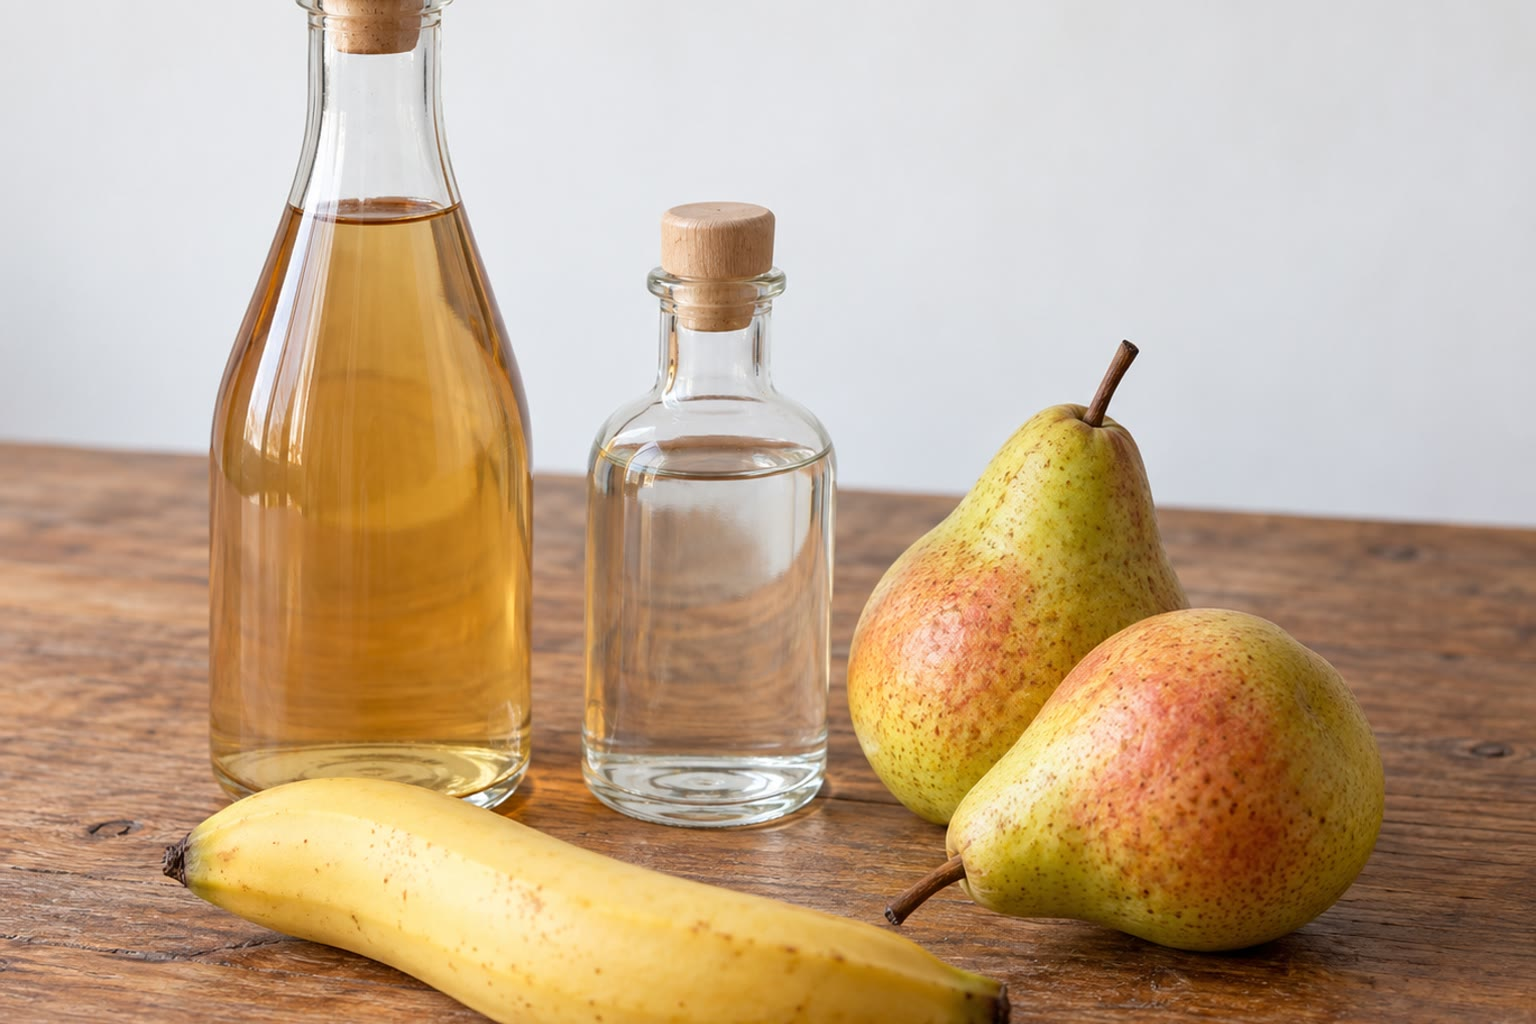
\includegraphics[width=0.5\linewidth]{images/book1/ai/g11-still-life-esters.jpg}

{\small الخل، \omterm{def:g6:solutions-and-solubility:solute}{ومذيب}، وفاكهة: كل رائحة تأتي من مجموعة مختلفة من \omterm{def:g7:atoms-and-molecules:atom}{الذرات} على هيكل
كربوني.}
\end{omfigure}

\section{المجموعات الوظيفية}

\begin{definition}[المجموعة الوظيفية]\label{def:g11:functional-groups:functional-group}
\emph{المجموعة الوظيفية}\index{مجموعة وظيفية} مجموعة من \omterm{def:g7:atoms-and-molecules:atom}{الذرات}، غير \omterm{def:g7:atoms-and-molecules:atom}{ذرات}
الكربون والهيدروجين في الهيكل المرتبطة بروابط أحادية فقط، تعطي \omterm{def:g7:atoms-and-molecules:molecule}{الجزيء} تفاعلاته
المميِّزة. والمركبات التي تشترك في مجموعة وظيفية تكوّن عائلة.
\end{definition}

\begin{omfigure}
\renewcommand{\arraystretch}{1.35}
\footnotesize
\begin{tabular}{@{}l@{\enspace}l@{\enspace}l@{\enspace}l@{\enspace}l@{}}
\hline
المجموعة & الصيغة & العائلة & نهاية الاسم & مثال \\
\hline
هيدروكسيل & \ce{-OH} & \omterm{def:g11:functional-groups:alcohol}{كحول} & \emph{-ول} & الإيثانول، \ce{CH3-CH2-OH} \\
كربونيل (طرفي) & \ce{-CHO} & \omterm{def:g11:functional-groups:carbonyl}{ألدهيد} & \emph{-ال} & الإيثانال، \ce{CH3-CHO} \\
كربونيل (داخلي) & \ce{C-CO-C} & \omterm{def:g11:functional-groups:carbonyl}{كيتون} & \emph{-ون} & البروبانون، \ce{CH3-CO-CH3} \\
كربوكسيل & \ce{-COOH} & \omterm{def:g11:functional-groups:carboxylic-acid}{حمض كربوكسيلي} & حمض \emph{\ldots-ويك} & حمض الإيثانويك، \ce{CH3-COOH} \\
\omterm{def:g11:functional-groups:carboxylic-acid}{إستر} & \ce{C-COO-C} & \omterm{def:g11:functional-groups:carboxylic-acid}{إستر} & \emph{\ldots-وات \ldots-يل} & إيثانوات الإيثيل، \ce{CH3-COO-CH2-CH3} \\
\omterm{def:g11:functional-groups:amine}{أمين} & \ce{-NH2} & \omterm{def:g11:functional-groups:amine}{أمين} & \emph{-أمين} & الإيثان \omterm{def:g11:functional-groups:amine}{أمين}، \ce{CH3-CH2-NH2} \\
\omterm{def:g11:functional-groups:amine}{أميد} & \ce{-CONH2} & \omterm{def:g11:functional-groups:amine}{أميد} & \emph{-أميد} & الإيثان \omterm{def:g11:functional-groups:amine}{أميد}، \ce{CH3-CONH2} \\
\omterm{def:g10:electron-shells:family}{هالوجين} & \ce{C-X} & \omterm{def:g11:functional-groups:halogenoalkane}{ألكان مهلجن} & البادئة \emph{كلورو-}، \ldots & كلورو ميثان، \ce{CH3Cl} \\
\omterm{def:g10:lewis-and-shape:multiple-bond}{رابطة ثنائية} & \ce{C=C} & \omterm{def:g11:functional-groups:halogenoalkane}{ألكين} & \emph{-ين} & الإيثين، \ce{CH2=CH2} \\
\hline
\end{tabular}\par\medskip

\setchemfig{atom sep=1.4em}
\begin{tabular}{@{}c@{\quad}c@{\quad}c@{\quad}c@{\quad}c@{}}
\chemfig{R-C(=[2]O)-H} & \chemfig{R-C(=[2]O)-R'} & \chemfig{R-C(=[2]O)-O-H} &
\chemfig{R-C(=[2]O)-O-R'} & \chemfig{R-C(=[2]O)-N(-[1]H)-[7]H} \\
\small \omterm{def:g11:functional-groups:carbonyl}{ألدهيد} & \small \omterm{def:g11:functional-groups:carbonyl}{كيتون} & \small \omterm{def:g11:functional-groups:carboxylic-acid}{حمض كربوكسيلي} & \small \omterm{def:g11:functional-groups:carboxylic-acid}{إستر} &
\small \omterm{def:g11:functional-groups:amine}{أميد}
\end{tabular}\par\medskip

{\small المجموعات الوظيفية الرئيسية، والخمس المبنية على مجموعة الكربونيل
\ce{C=O}، مرسومة كاملة. يرمز R وR$'$ إلى سلاسل كربونية (مجموعات
ألكيل) وX إلى \omterm{def:g7:atoms-and-molecules:atom}{ذرة} \omterm{def:g10:electron-shells:family}{هالوجين} (F، Cl، Br، I).}
\end{omfigure}

\section{الكحولات وصنفها}

\begin{definition}[الكحول، وصنف الكحول]\label{def:g11:functional-groups:alcohol}
\emph{الكحول}\index{كحول} له مجموعة هيدروكسيل \ce{-OH} مرتبطة \omterm{def:g7:atoms-and-molecules:atom}{بذرة} كربون
ليس لها إلا روابط أحادية. و\emph{صنف الكحول}\index{صنف الكحول} أولي أو ثانوي أو
ثالثي بحسب ارتباط \omterm{def:g7:atoms-and-molecules:atom}{ذرة} الكربون الحاملة للمجموعة \ce{-OH} \omterm{def:g7:atoms-and-molecules:atom}{بذرة} كربون أخرى أو
اثنتين أو ثلاث. (والميثانول، \ce{CH3OH}، الذي لا يرتبط كربونه بأي كربون،
يُعدّ مع الكحولات الأولية.)
\end{definition}

\begin{omfigure}
\setchemfig{atom sep=1.9em}
\begin{tabular}{ccc}
\chemfig{-[:30]-[:-30]-[:30]-[:-30]OH} &
\chemfig{-[:30](-[:90]OH)-[:-30]-[:30]} &
\chemfig{-[:0](-[:90]OH)(-[:-90])-[:0]} \\[4pt]
\small بوتان-1-ول & \small بوتان-2-ول & \small 2-ميثيل بروبان-2-ول \\
\small \textbf{أولي} & \small \textbf{ثانوي} & \small \textbf{ثالثي} \\
\small (لكربون \ce{-OH} جار كربوني واحد) & \small (جاران) &
\small (ثلاثة جيران)
\end{tabular}

{\small ثلاثة \omterm{def:g11:organic-skeletons:isomer}{متماكبات} للصيغة \ce{C4H10O}، وثلاثة أصناف من \omterm{def:g11:functional-groups:alcohol}{الكحول}.}
\end{omfigure}

\section{الألدهيدات والكيتونات والأحماض والإسترات}

\begin{definition}[الألدهيد والكيتون]\label{def:g11:functional-groups:carbonyl}
مجموعة الكربونيل \omterm{def:g10:lewis-and-shape:multiple-bond}{رابطة ثنائية} \ce{C=O}. فإذا كانت \omterm{def:g7:atoms-and-molecules:atom}{ذرة} كربونها في طرف السلسلة
(مرتبطة \omterm{def:g7:atoms-and-molecules:atom}{بذرة} هيدروجين واحدة على الأقل) كان المركب
\emph{ألدهيدًا}\index{ألدهيد}؛ وإذا كانت داخل السلسلة (مرتبطة بذرتي كربون) كان
المركب \emph{كيتونًا}\index{كيتون}.
\end{definition}

\begin{definition}[الحمض الكربوكسيلي والإستر]\label{def:g11:functional-groups:carboxylic-acid}
\emph{الحمض الكربوكسيلي}\index{حمض كربوكسيلي} له مجموعة كربوكسيل
\ce{-COOH}، أي كربونيل وهيدروكسيل على \omterm{def:g7:atoms-and-molecules:atom}{ذرة} الكربون نفسها. و\emph{الإستر}\index{إستر}
له المجموعة \ce{-COO-} بين سلسلتين كربونيتين: وهو قريب من حمض حلّت محلَّ مجموعته
\ce{-OH} مجموعةُ \ce{-O-}R$'$ آتية من \omterm{def:g11:functional-groups:alcohol}{كحول}.
\end{definition}

\begin{example}[إيثانوات الإيثيل]\label{ex:g11:functional-groups:ethyl-ethanoate}
\omterm{def:g6:solutions-and-solubility:solute}{للمذيب} إيثانوات الإيثيل، \ce{CH3-COO-CH2-CH3}، رائحة حلوى الإجاص ومزيل طلاء
الأظافر. «جزؤه الحمضي»، \ce{CH3-CO}، يأتي من حمض الإيثانويك \ce{CH3-COOH}
ويعطي الكلمة الأولى من الاسم، \emph{إيثانوات}؛ و«جزؤه الكحولي»،
\ce{O-CH2-CH3}، يأتي من الإيثانول \ce{CH3-CH2-OH} ويعطي الكلمة الثانية،
\emph{الإيثيل}. ويبيّن فصل لاحق كيف يُصنع \omterm{def:g11:functional-groups:carboxylic-acid}{الإستر} من حمضه
وكحوله.
\end{example}

\begin{omfigure}
\setchemfig{atom sep=2.2em}
\chemfig{@{a}H_3C-@{c}C(=[2]@{o}O)-@{x}O-CH_2-@{z}CH_3}
\chemmove{
  \fill[omProp, opacity=0.14, rounded corners]
    ($(a.south west)+(-0.12,-0.15)$) rectangle ($(o.north east)+(0.25,0.12)$);
  \fill[omDef, opacity=0.14, rounded corners]
    ($(x.south west)+(-0.2,-0.15)$) rectangle ($(z.north east)+(0.4,0.75)$);
  \node[omProp, anchor=north east, align=right, font=\small] at ($(c.south)+(0.15,-0.25)$)
    {الجزء الحمضي، من حمض الإيثانويك:\\ \emph{إيثانوات}};
  \node[omDef, anchor=north west, align=left, font=\small] at ($(x.south)+(0.05,-0.25)$)
    {الجزء الكحولي، من الإيثانول:\\ \emph{الإيثيل}};}
\par\vspace{1.4cm}

{\small تسمية \omterm{def:g11:functional-groups:carboxylic-acid}{الإستر}: الجزء الكحولي يعطي اسم ألكيل
(\emph{الإيثيل})، والجزء الحمضي اسمًا ينتهي بالمقطع \emph{-وات}
(\emph{إيثانوات})؛ والاسم «إيثانوات الإيثيل».}
\end{omfigure}

\section{الأمينات والأميدات والألكانات المهلجنة والألكينات}


\begin{definition}[الأمين والأميد]\label{def:g11:functional-groups:amine}
\emph{الأمين}\index{أمين} له \omterm{def:g7:atoms-and-molecules:atom}{ذرة} نيتروجين مرتبطة بسلسلة كربونية
برابطة أحادية، كما في \ce{-NH2}. و\emph{الأميد}\index{أميد} له \omterm{def:g7:atoms-and-molecules:atom}{ذرة} نيتروجين
مرتبطة بكربون مجموعة كربونيل، كما في \ce{-CO-NH2}.
\end{definition}

\begin{definition}[الألكان المهلجن والألكين]\label{def:g11:functional-groups:halogenoalkane}
\emph{الألكان المهلجن}\index{ألكان مهلجن} \omterm{def:g11:organic-skeletons:alkane}{ألكان} استُبدلت فيه \omterm{def:g7:atoms-and-molecules:atom}{بذرة} هيدروجين
أو أكثر \omterm{def:g7:atoms-and-molecules:atom}{ذرات} \omterm{def:g10:electron-shells:family}{هالوجين} (F، Cl، Br، I). و\emph{الألكين}\index{ألكين} له \omterm{def:g10:lewis-and-shape:multiple-bond}{رابطة
ثنائية} كربون--كربون، \ce{C=C}.
\end{definition}

\begin{remark}[الروائح والمجموعات]\label{rem:g11:functional-groups:smells}
كثير من الأمينات الصغيرة رائحتها رائحة السمك الفاسد، ورائحة السمك الذي فقد طزاجته
ترجع في معظمها إليها. وكثير من \omterm{def:g11:functional-groups:carboxylic-acid}{الإسترات} الصغيرة رائحتها رائحة الفاكهة. والأحماض
الكربوكسيلية الصغيرة رائحتها لاذعة، كالخل؛ والبروبانون، وهو \omterm{def:g11:functional-groups:carbonyl}{كيتون}، هو رائحة
\omterm{def:g6:solutions-and-solubility:solute}{المذيب} المألوفة لمزيل طلاء الأظافر.
\end{remark}

\section{التسمية}

\begin{method}[تسمية مركب عضوي ذي مجموعة وظيفية واحدة]\label{met:g11:functional-groups:naming}
\begin{enumerate}
  \item جد أطول سلسلة كربونية \emph{تحوي} كربون
        \omterm{def:g11:functional-groups:functional-group}{المجموعة الوظيفية} (أو، \omterm{def:g11:functional-groups:alcohol}{للكحول} \omterm{def:g11:functional-groups:amine}{والأمين}، الكربون
        الحامل لها): فهي تعطي الجذر.
  \item رقّم السلسلة من الطرف الذي يعطي \omterm{def:g11:functional-groups:functional-group}{المجموعة الوظيفية}
        أصغر رقم.
  \item ألحق باسم \omterm{def:g11:organic-skeletons:alkane}{الألكان} \emph{نهاية} العائلة،
        مسبوقة بموقع المجموعة إن لزم: بروبان-2-ول،
        بوتان-2-ون. (فالألدهيدات والأحماض والأميدات مجموعتها على
        الكربون 1: فلا رقم.)
  \item أضف المستبدِلات الألكيلية بوادئ، مع مواقعها،
        كما في الألكانات؛ \omterm{def:g10:electron-shells:family}{والهالوجين} بادئة دائمًا (2-كلورو بروبان).
\end{enumerate}
\end{method}

\begin{example}[أربعة أسماء]\label{ex:g11:functional-groups:names}
\setchemfig{atom sep=1.7em}
\chemfig{-[:30](-[:90]OH)-[:-30]} هو بروبان-2-ول (\omterm{def:g11:functional-groups:alcohol}{كحول} ثانوي)؛
\chemfig{-[:30](=[:90]O)-[:-30]-[:30]} هو بوتان-2-ون؛
\chemfig{-[:30]-[:-30]-[:30](=[:90]O)-[:-30]OH} هو حمض البوتانويك؛
\chemfig{-[:30](-[:90])-[:-30]-[:30]=[:-30]O} هو 3-ميثيل بوتانال.
\end{example}

\begin{omfigure}
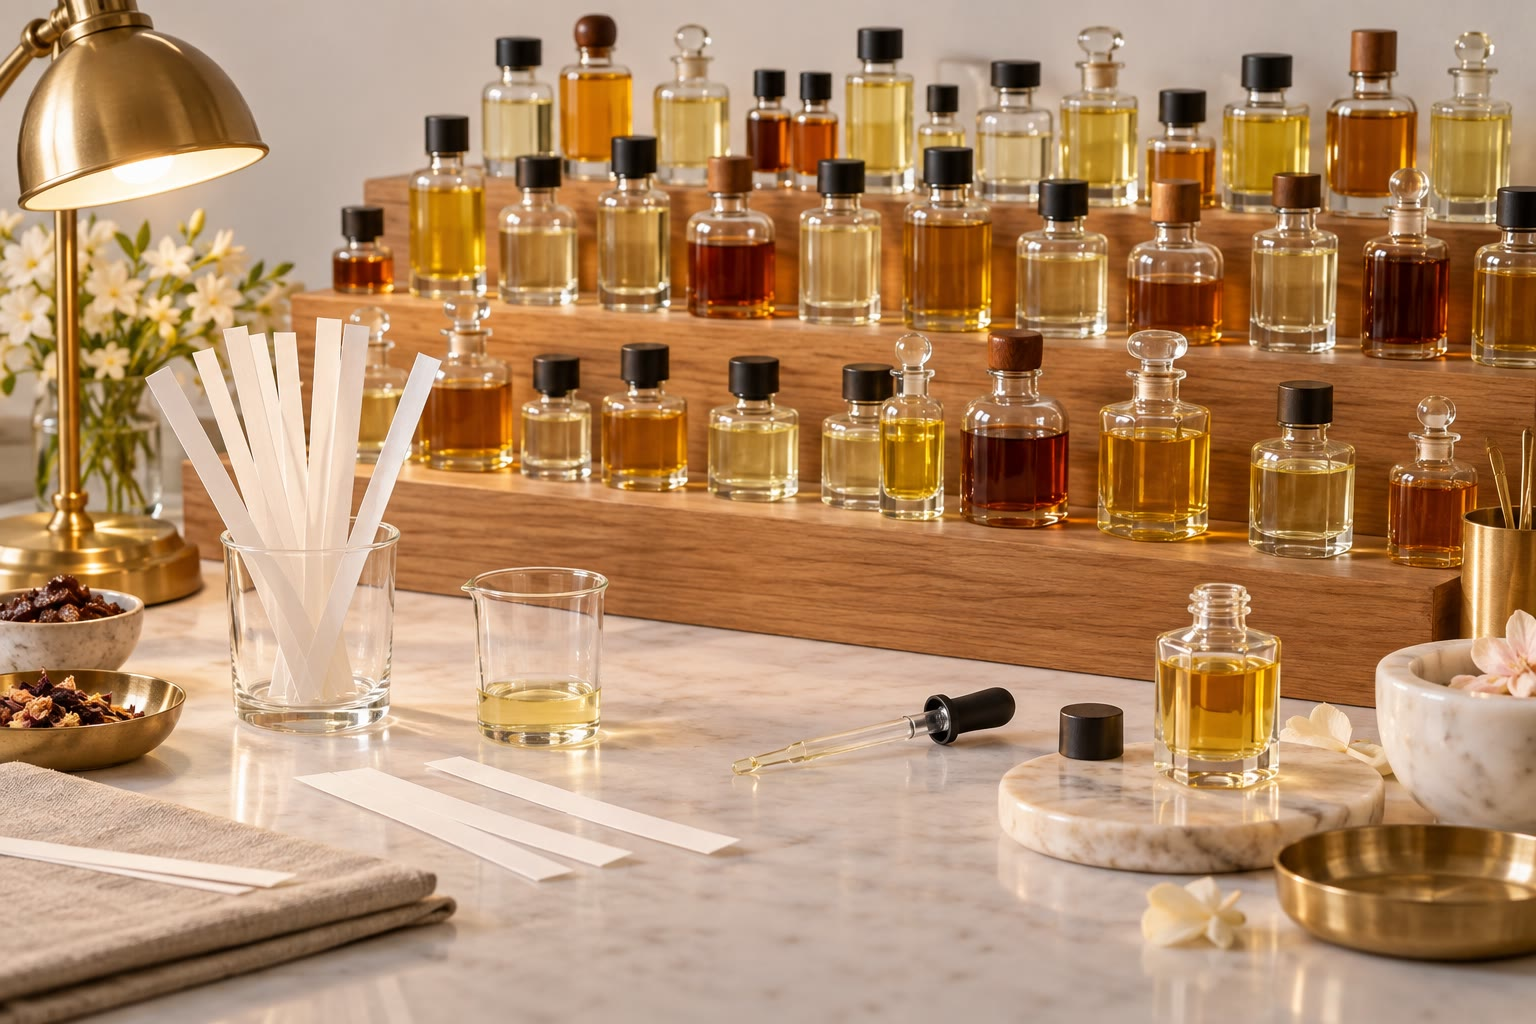
\includegraphics[width=0.48\linewidth]{images/book1/ai/g11-perfumer-lab.jpg}

{\small طاولة صانع عطور: كثير من القوارير تحوي \omterm{def:g11:functional-groups:carboxylic-acid}{إسترات} \omterm{def:g11:functional-groups:alcohol}{وكحولات}
وألدهيدات وكيتونات.}
\end{omfigure}

\begin{safety}{\ghs[0.82cm]{GHS02}\ghs[0.82cm]{GHS05}\ghs[0.82cm]{GHS07}}
% ledger: ghs:acetone, ghs:acetic-acid
البروبانون شديد القابلية للاشتعال ومهيّج للعينين؛ وبخاره يسبب النعاس. وحمض
الإيثانويك الخالص قابل للاشتعال ويسبب حروقًا شديدة للجلد والعينين؛ والخل \omterm{def:g2:mixing-and-dissolving:dissolve}{محلول}
مخفف منه. ولا تُختبر الروائح أبدًا بشم الدورق: بل يُدفع البخار برفق نحو الأنف
باليد، ولا يكون ذلك إلا حين يأذن
المعلم.
\end{safety}

\section{تمارين}


\begin{exercise}[$\star$]\label{exo:g11:functional-groups:1}
سمِّ \omterm{def:g11:functional-groups:functional-group}{المجموعة الوظيفية} وعائلة كل مركب:
\ce{CH3-CH2-CH2-OH}؛ \ce{CH3-CO-CH2-CH3}؛ \ce{CH3-CH2-COOH}؛
\ce{CH3-COO-CH3}؛ \ce{CH3-CH2-NH2}.
\end{exercise}

\begin{exercise}[$\star$]\label{exo:g11:functional-groups:2}
سمِّ: \ce{CH3-OH}؛ \ce{CH3-CH2-CH2-OH}؛ \ce{HCOOH}؛ \ce{CH3-CH2-CHO}؛
\ce{CH3-CO-CH3}.
\end{exercise}

\begin{exercise}[$\star$]\label{exo:g11:functional-groups:3}
إلى أي عائلة ينتمي كل مركب: بوتان-2-ول، والبنتانال، وبروبانوات
الميثيل، والبروبان \omterm{def:g11:functional-groups:amine}{أميد}، و2-برومو بروبان، وبوت-1-ين؟
\end{exercise}

\begin{exercise}[$\star$]\label{exo:g11:functional-groups:4}
اكتب الصيغتين نصف البنيويتين للبروبانال وللبروبانون. أيهما \omterm{def:g11:functional-groups:carbonyl}{الألدهيد}؟
وكيف تعرف ذلك؟
\end{exercise}

\begin{exercise}[$\star$]\label{exo:g11:functional-groups:5}
أعطِ صنف كل من بروبان-1-ول، وبروبان-2-ول، و2-ميثيل بروبان-2-ول.
\end{exercise}

\begin{exercise}[$\star\star$]\label{exo:g11:functional-groups:6}
ارسم الصيغ الهيكلية للمركبات بنتان-3-ول، وحمض 2-ميثيل البوتانويك،
وهكسان-2-ون، وإيثانوات البروبيل.
\end{exercise}

\begin{exercise}[$\star\star$]\label{exo:g11:functional-groups:7}
للبروبانال والبروبانون \omterm{def:g11:organic-skeletons:formulas}{الصيغة الجزيئية} نفسها. أعطها. وهل
هما متماكبان؟ وهل لهما \omterm{def:g11:functional-groups:functional-group}{المجموعة الوظيفية} نفسها؟
\end{exercise}

\begin{exercise}[$\star\star$]\label{exo:g11:functional-groups:8}
اكتب \omterm{def:g11:organic-skeletons:formulas}{الصيغة نصف البنيوية} واسم \omterm{def:g11:functional-groups:carboxylic-acid}{الإستر} الذي يأتي جزؤه الحمضي من حمض الميثانويك
\ce{HCOOH} ويأتي جزؤه الكحولي من الإيثانول؛ ثم \omterm{def:g11:functional-groups:carboxylic-acid}{الإستر} المصنوع من حمض الإيثانويك
وبروبان-1-ول.
\end{exercise}

\begin{exercise}[$\star\star$]\label{exo:g11:functional-groups:9}
سمِّ \omterm{def:g11:functional-groups:carboxylic-acid}{الإسترات} \ce{CH3-COO-CH3} و\ce{CH3-CH2-COO-CH2-CH3}
و\ce{HCOO-CH3}، وأعطِ الحمض \omterm{def:g11:functional-groups:alcohol}{والكحول} اللذين يرتبط بهما كل منها.
\end{exercise}

\begin{exercise}[$\star\star$]\label{exo:g11:functional-groups:10}
ارسم وسمِّ \omterm{def:g11:functional-groups:alcohol}{الكحولات} الأربعة ذات الصيغة \ce{C4H10O}، وأعطِ
صنف كل منها.
\end{exercise}

\begin{exercise}[$\star\star$]\label{exo:g11:functional-groups:11}
مستعينًا بجدول المجموعات: ما عائلة \ce{CH3-CO-NH2}؟ وبأي
نهاية ينتهي اسم \omterm{def:g11:functional-groups:halogenoalkane}{الألكين}؟ وأي العائلات لها مجموعة
كربونيل وعلى الكربون نفسه \omterm{def:g7:atoms-and-molecules:atom}{ذرة} أكسجين أو نيتروجين؟
\end{exercise}

\begin{exercise}[$\star\star\star$]\label{exo:g11:functional-groups:12}
أحط بدائرة وسمِّ المجموعات الوظيفية للأسبرين وللباراسيتامول.
(المجموعة \ce{-OH} المرتبطة مباشرة بحلقة مثل حلقة الباراسيتامول تسمى
مجموعة فينول؛ وسلوكها مختلف عن سلوك \omterm{def:g11:functional-groups:alcohol}{الكحول}.)
\begin{center}
\setchemfig{atom sep=1.6em}
\chemfig{*6(-=-(-COOH)=(-O-[:150]C(=[:90]O)-[:210]H_3C)-=)}
\qquad
\chemfig{*6((-OH)=-=(-N(-[2]H)-[7]C(=[6]O)-[1]CH_3)-=-)}
\\[2pt] \small الأسبرين \hspace{4.2cm} الباراسيتامول
\end{center}
\end{exercise}

\begin{exercise}[$\star\star\star$]\label{exo:g11:functional-groups:13}
% ledger: bp:C2H5OH, bp:CH3OCH3
للإيثانول \ce{CH3-CH2-OH} والميثوكسي ميثان \ce{CH3-O-CH3} \omterm{def:g11:organic-skeletons:formulas}{الصيغة
الجزيئية} نفسها. أعطها. والميثوكسي ميثان ينتمي إلى عائلة ليست في
الجدول، هي الإيثرات. أي الاثنين يستطيع أن يكوّن روابط هيدروجينية بين
جزيئاته؟ وأيهما يغلي عند درجة أعلى (أحدهما يغلي عند \qty{78}{\celsius}،
والآخر عند \qty{-25}{\celsius})؟
\end{exercise}

\begin{exercise}[$\star\star\star$]\label{exo:g11:functional-groups:14}
حمض اللبنيك، الذي تصنعه العضلات المتعبة، هو
\chemfig{CH_3-CH(-[2]OH)-COOH}. سمِّ مجموعتيه الوظيفيتين. وحين يكون في
\omterm{def:g7:atoms-and-molecules:molecule}{الجزيء} مجموعة حمضية ومجموعة أخرى، يعطي الحمضُ النهايةَ وتصير المجموعة الأخرى بادئة
(\emph{هيدروكسي-} للمجموعة \ce{-OH}، و\emph{أمينو-} للمجموعة
\ce{-NH2}). سمِّ حمض اللبنيك، ثم الغليسين،
\ce{H2N-CH2-COOH}.
\end{exercise}

\begin{exercise}[$\star\star\star$]\label{exo:g11:functional-groups:15}
يتحول النبيذ المتروك في \omterm{def:g4:air-a-mixture-of-gases:air}{الهواء} إلى خل: فيصير الإيثانول حمض إيثانويك، مرورًا
بالإيثانال. اكتب الصيغ نصف البنيوية والجزيئية للمركبات الثلاثة وعائلاتها.
وماذا يتغير في الصيغة في كل
خطوة؟
\end{exercise}

\section{مسألة: نكهات الفاكهة}

\begin{problem}[{مسألة نهاية الأسبوع --- كيميائية نكهات تبني رائحة الموز: ما
الكتلة المولية للجزيء الأساسي؟}]
\label{pb:g11:functional-groups:1}
% ledger: aw:C, aw:H, aw:O
لدى كيميائية نكهات خمسة مركبات على طاولتها:
\begin{center}
\begin{tabular}{ll}
A & \chemfig{CH_3-C(=[2]O)-O-CH_2-CH_2-CH(-[2]CH_3)-CH_3} \\[16pt]
B & \chemfig{HO-CH_2-CH_2-CH(-[2]CH_3)-CH_3} \\[10pt]
C & \ce{CH3-COOH} \\
D & \ce{CH3-CH2-CH2-CH2-CH2-CHO} \\
E & \ce{CH3-CH2-CH2-COO-CH2-CH3}
\end{tabular}
\end{center}
للمركب A رائحة الموز وحلوى الإجاص، وللمركب B رائحة الشعير المنبت، وللمركب C
رائحة الخل، وللمركب D رائحة العشب المقصوص، وللمركب E رائحة الأناناس.

\medskip
\noindent\textbf{الجزء الأول --- المجموعات والعائلات.}
\begin{enumerate}
  \item سمِّ \omterm{def:g11:functional-groups:functional-group}{المجموعة الوظيفية} لكل مركب.
  \item أعطِ عائلة كل منها.
  \item أي المركبات \omterm{def:g11:functional-groups:carboxylic-acid}{إسترات}؟ وما روائحها؟
  \item ما \omterm{def:g11:functional-groups:alcohol}{صنف الكحول} B؟
  \item أعطِ \omterm{def:g11:organic-skeletons:formulas}{الصيغة الجزيئية} للمركب D، وارسم متماكبًا له
        يكون \omterm{def:g11:functional-groups:carbonyl}{كيتونًا}.
\end{enumerate}

\medskip
\noindent\textbf{الجزء الثاني --- الأسماء.}
\begin{enumerate}[resume]
  \item سمِّ B (جد أطول سلسلة تحوي الكربون الحامل
        للمجموعة \ce{-OH}).
  \item سمِّ C وD.
  \item سمِّ E، وأعطِ الحمض \omterm{def:g11:functional-groups:alcohol}{والكحول} اللذين يرتبط بهما.
  \item اشرح اسم A، إيثانوات 3-ميثيل البوتيل: أي جزء يأتي
        من الحمض، وأيهما من \omterm{def:g11:functional-groups:alcohol}{الكحول}؟
\end{enumerate}

\medskip
\noindent\textbf{الجزء الثالث --- من حمض \omterm{def:g11:functional-groups:alcohol}{وكحول}.}
\begin{enumerate}[resume]
  \item بأي مركبين من مركبات الطاولة يرتبط A؟
  \item أعطِ الصيغ الجزيئية للمركبات A وB وC.
  \item يُصنع \omterm{def:g11:functional-groups:carboxylic-acid}{الإستر} من حمضه وكحوله مع فقد \omterm{def:g7:atoms-and-molecules:molecule}{جزيء} صغير
        واحد. جد هذا \omterm{def:g7:atoms-and-molecules:molecule}{الجزيء} مستعينًا بالصيغ.
  \item اكتب معادلة تكوّن A، بالصيغ الجزيئية،
        وتحقق من أنها موزونة.
\end{enumerate}

\medskip
\noindent\textbf{الجزء الرابع --- الكتل المولية.}
\begin{enumerate}[resume]
  \item احسب الكتلتين الموليتين للمركبين B وC.
  \item استنتج \omterm{def:g10:the-mole:molar-mass}{الكتلة المولية} للمركب A من معادلة السؤال 13.
  \item احسب \omterm{def:g10:the-mole:molar-mass}{الكتلة المولية} للمركب A مباشرة من صيغته،
        وقارن.
  \item وُجد أن لعيّنة فاكهية مجهولة \omterm{def:g10:the-mole:molar-mass}{كتلة مولية} قريبة من
        \qty{116}{g/mol}. هل هي A أم E؟
  \item لحمض الهبتانويك، \ce{CH3-(CH2)5-COOH}، رائحة زنخة. بيّن أنه
        متماكب للمركب A. وهل تكفي \omterm{def:g10:the-mole:molar-mass}{الكتلة المولية} وحدها للتعرف على مركب؟
  \item لماذا يقول الكيميائيون إن الرائحة تتبع \omterm{def:g11:functional-groups:functional-group}{المجموعة الوظيفية} بقدر ما تتبع
        الهيكل؟ استعن بالمركب A وحمض الهبتانويك.
  \item اذكر الجواب النهائي: ما \omterm{def:g10:the-mole:molar-mass}{الكتلة المولية} \omterm{def:g11:functional-groups:carboxylic-acid}{لإستر} الموز،
        إيثانوات 3-ميثيل البوتيل؟
\end{enumerate}
\end{problem}
